\documentclass[letterpaper]{article}
\usepackage{aaai2026}
\nocopyright
\usepackage{times}
\usepackage{helvet}
\usepackage{courier}
\usepackage[hyphens]{url}
\usepackage{graphicx}
\usepackage{placeins}
\urlstyle{rm}
\def\UrlFont{\rm}
\usepackage{natbib}
\usepackage{caption}
\frenchspacing
\setlength{\pdfpagewidth}{8.5in}
\setlength{\pdfpageheight}{11in}

\usepackage{amsmath,amssymb}
\usepackage{booktabs}
\usepackage{tabularx}
\usepackage{iftex}
\ifXeTeX
  \makeatletter
  \@ifpackageloaded{fontspec}{}{\usepackage{fontspec}}
  \makeatother
  \usepackage{xeCJK}
  \xeCJKsetup{CJKspace=true}
  \defaultfontfeatures{Ligatures=TeX}
  \IfFontExistsTF{TeX Gyre Termes}{%
    \setmainfont{TeX Gyre Termes}%
  }{%
    \IfFontExistsTF{Times New Roman}{%
      \setmainfont{Times New Roman}%
    }{%
      \setmainfont{STIX Two Text}%
    }%
  }
  \IfFontExistsTF{NanumBarunGothicOTF}{%
    \setCJKmainfont[
      ItalicFont={NanumBarunGothicOTF},
      SmallCapsFont={NanumBarunGothicOTF}
    ]{NanumBarunGothicOTF}%
    \setCJKsansfont{NanumBarunGothicOTF}%
    \setCJKmonofont{NanumBarunGothicOTF}%
  }{%
    \IfFontExistsTF{Noto Sans CJK KR}{%
      \setCJKmainfont[
        ItalicFont={Noto Sans CJK KR},
        SmallCapsFont={Noto Sans CJK KR}
      ]{Noto Sans CJK KR}%
      \setCJKsansfont{Noto Sans CJK KR}%
      \setCJKmonofont{Noto Sans CJK KR}%
    }{%
      \setCJKmainfont[
        Scale=0.92,
        ItalicFont={Apple SD Gothic Neo},
        SmallCapsFont={Apple SD Gothic Neo}
      ]{Apple SD Gothic Neo}%
      \setCJKsansfont[Scale=0.92]{Apple SD Gothic Neo}%
      \setCJKmonofont[Scale=0.92]{Apple SD Gothic Neo}%
    }%
  }
  \xeCJKDeclareCharClass{Default}{"00B7}
\else
  \usepackage{kotex}
\fi

\newif\ifanonymoussubmission
\ifdefined\ANONBUILD
  \anonymoussubmissiontrue
\else
  \anonymoussubmissionfalse
\fi

\newcommand{\system}{TRACE-RPG}
\newcommand{\Valid}{\mathrm{valid}}
\newcommand{\AcceptSet}{\mathcal{A}}
\newcommand{\GoalSet}{\mathcal{G}}
\newcommand{\HitSet}{\mathcal{H}}
\newcommand{\SchemaSet}{\mathcal{S}}
\newcommand{\RepoURL}{\ifanonymoussubmission [Anonymous Repository URL withheld for double-anonymous review]\else \url{https://github.com/akillness/neural_symbolic_in_game}\fi}
\AtBeginDocument{\emergencystretch=2.5em}
\providecommand{\Description}[2][]{}

\anonymoussubmissionfalse

\setcounter{secnumdepth}{1}

\title{TRACE-RPG: 서사 중재와 게임 상태 권한 부여를 위한 감사 가능한 제안--커밋 경계}
\author{
  정장영\textsuperscript{\rm 1},
  강신진\textsuperscript{\rm 2}\thanks{교신저자.}
}
\affiliations{
  \textsuperscript{\rm 1}홍익대학교 게임학과\\
  \textsuperscript{\rm 2}홍익대학교
}

\begin{document}
\maketitle

\begin{abstract}
스키마에 부합하는 게임 내 행동 제안이라도 접근할 수 없는 물체, 비인가 전이, 조기 비밀 공개를 포함할 수 있다. \system{}는 형식 정리 1--4로 뒷받침된 결정론적 7술어 게이트에서 제안 권한과 커밋 권한을 분리한다. 1,664건 유한 그래프 감사에서 의미 게이트는 스키마 전용 대조군의 위험 커밋 260/416건을 0/416건으로 차단했고(오탐 0/156, 수리 128/260), 48건 다중 홉 폐쇄에서 60/60 동률을 돌파했다(\texttt{ontology\_}\allowbreak\texttt{multihop\_}\allowbreak\texttt{gate} 48/48 대 평면 20/48). 3개 퀘스트 24에피소드 라이브 Gemini 평가에서 위험 커밋 0/129건과 리플레이 24/24건을 달성했고(70턴 차단, 리비전 미인증), 2차 한·영 우회 검증기는 97.2\% 재현율·0.0\% 오거부를 기록하며 \texttt{TR01--TR06} 인간 평가 패킷(\texttt{AWAITING\_}\allowbreak\texttt{HUMAN\_}\allowbreak\texttt{RATERS})을 구축했다.
\end{abstract}

\section{서론}
스키마에 부합하는 게임 내 행동 제안이라도 접근할 수 없는 물체를 요구하거나 권한이 없는 상태 전이, 혹은 현재 시점에서 공개할 수 없는 비밀 발화를 포함할 수 있다. 서사적 정합성(grounding)과 개연성 있는 대화 생성 \cite{S03_weir2024ontologically,S20_ashby2023personalized}은 후보 콘텐츠를 제공할 뿐이며, 게임 엔진은 현재 상태에서 어떤 전이를 승인할지 별도로 판정해야 한다.

\system{}는 이 판정을 외부의 제안--커밋(proposal-to-commit) 경계에서 강제한다(그림~\ref{fig:architecture}). 모델과 어댑터가 구조화된 후보를 제출하면 결정론적 게이트가 행동 정책, 선행조건, 물체 도달 가능성, NPC 지식, 정보 공개 권한, 효과, 퀘스트 단계 단조성을 검사한다. 검사에 실패하면 게이트는 제한된 수리를 위한 구조화된 오류를 반환하며, 수리는 정본 상태(canonical state)가 아닌 후보만 수정하고 동일 상태 재검증을 통과한 경우에만 상태를 갱신한다. 여덟 역할 읽기 전용 온톨로지 뷰는 쓰기 권한 없이 출처 선언과 검사·결정을 연결하며, 해시 연결 전이 기록은 의미적 리플레이와 배정 전수 회계(assignment-complete accounting)를 보장한다.

개념적으로 이 계약은 단순 사실 일치(factual grounding)를 넘어 NPC의 \emph{인식론적 지식 경계}(행위자가 알고 있는 사실)와 \emph{정보 공개 권한 정책}(현재 퀘스트 단계에서 발화할 수 있는 사실)을 분리한다. 방법론적으로는 LLM 호출이 0회인 결정론적 검증 계층(게이트 검사, 유도 수리, 엔진 리플레이)과 실패를 누락 없이 보존하는 제한된 확률적 제안기 계층을 엄격히 분리한다.

결정론적 감사에서 스키마 전용 대조군은 32개 유한 그래프 조합에 걸쳐 기준상 무효인 제안 260/416건을 커밋한 반면, 모든 의미 게이트 조건은 0/416건을 기록했고 최초 유효 제안 156/156건(오탐 0/156) 및 고유 구조 서명 11/11종을 모두 보존했다. 반례 유도 수리는 최초 무효 제안 260건 중 128건을 유효 커밋으로 복구했다. 단일 홉 정보 공개 검사에서도 일반 규칙과 온톨로지 게이트는 60/60건 일치하며 위험 공개 51건을 차단했고, 후속 48건 다중 홉 폐쇄 벤치마크에서는 양자를 뚜렷이 구분한다(\texttt{ontology\_}\allowbreak\texttt{multihop\_}\allowbreak\texttt{gate} 48/48 대 \texttt{flat\_}\allowbreak\texttt{1hop\_}\allowbreak\texttt{rule} 20/48, 위험 누출 28건 차단). 여기에 확장 0-LLM 감사, 불변식 \textbf{I1--I4}에 대한 형식 정리 1--4, 24에피소드 라이브 다중 퀘스트 Gemini 평가(2종 모델, 3개 월드, 위험 커밋 0건, 엄격 리플레이 24/24), 2차 한·영 우회 검증기(우회 재현율 97.2\% 및 양성 오거부 0.0\%), 그리고 실제 트레이스 결속 36항목 블라인드 인간 평가 패킷(\texttt{AWAITING\_}\allowbreak\texttt{HUMAN\_}\allowbreak\texttt{RATERS})과 Croissant~1.0 메타데이터를 더해 재현 가능한 공개 경계를 완성한다.

\section{관련 연구와 연구 공백}
정합성, 기억, 계획, 역할 기반 에이전트 \cite{S03_weir2024ontologically,S20_ashby2023personalized,S07_park2023generative,S08_shao2023character} 및 플레이어·대화 시스템 \cite{S21_akoury2023player,S22_hochreiter2026beyond,S23_yin2026contextualized,S02_figueiredo2025scaffolded}은 맥락적 상호작용을 지원하는 반면, 본 연구는 인코딩된 현재 상태와 공개 정책이 제안된 전이를 허용하는지를 판정한다. 정서 및 몰입 모델링 \cite{S24_yannakakis2011experiencedriven,S25_melhart2020engagement,S26_wang2026engagement}은 생성 스타일을 안내할 뿐 상태 변경 권한을 부여하지 않는다.

기존 벤치마크와 자동 플레이테스팅은 상태, 체화 환경, 콘텐츠, 과정, 사회적 상호작용, 장기 과업을 다루며 \cite{S11_cote2019textworld,S12_wang2022scienceworld,S13_fan2022minedojo,S14_perezliebana2019gvgai,S15_liu2024agentbench,S16_ma2024agentboard,S17_zhou2024sotopia,S18_paglieri2025balrog,S19_lepelletier2022playtesting}, NCP-Bench는 서사적 일관성과 사실 정합성을 평가한다 \cite{S58_ma2026ncpbench}. 문법·스키마·어포던스·규칙 기반 기법 \cite{S09_geng2023grammar,S10_beurerkellner2023prompting,S36_scholak2021picard,S50_kambhampati2024llmmodulo,S51_ichter2023saycan,S52_wang2025agentspec,S53_li2025settingdc,S54_zhou2025story2game,S42_buongiorno2024pangea}, 반례 기반 수리 \cite{S45_madaan2023selfrefine,S48_shinn2023reflexion,S46_chen2023selfdebug,S47_solarlezama2006sketching}, 재현성·리플레이 표준 \cite{S31_agarwal2021precipice,S33_pineau2021reproducibility,S56_feng2025agentrr,S59_sun2025bdc}이 본 설계의 토대다. 스키마 적합성과 행위 합법성, 또는 사실 정합성과 발화 안전성을 동일시하던 선행 연구와 달리, \system{}는 스키마 파싱, 인식론적 지식, 공개 권한, 정본 상태 커밋을 독립 감사 가능한 게이트로 분리한다.


\begin{figure*}[!t]
  \centering
  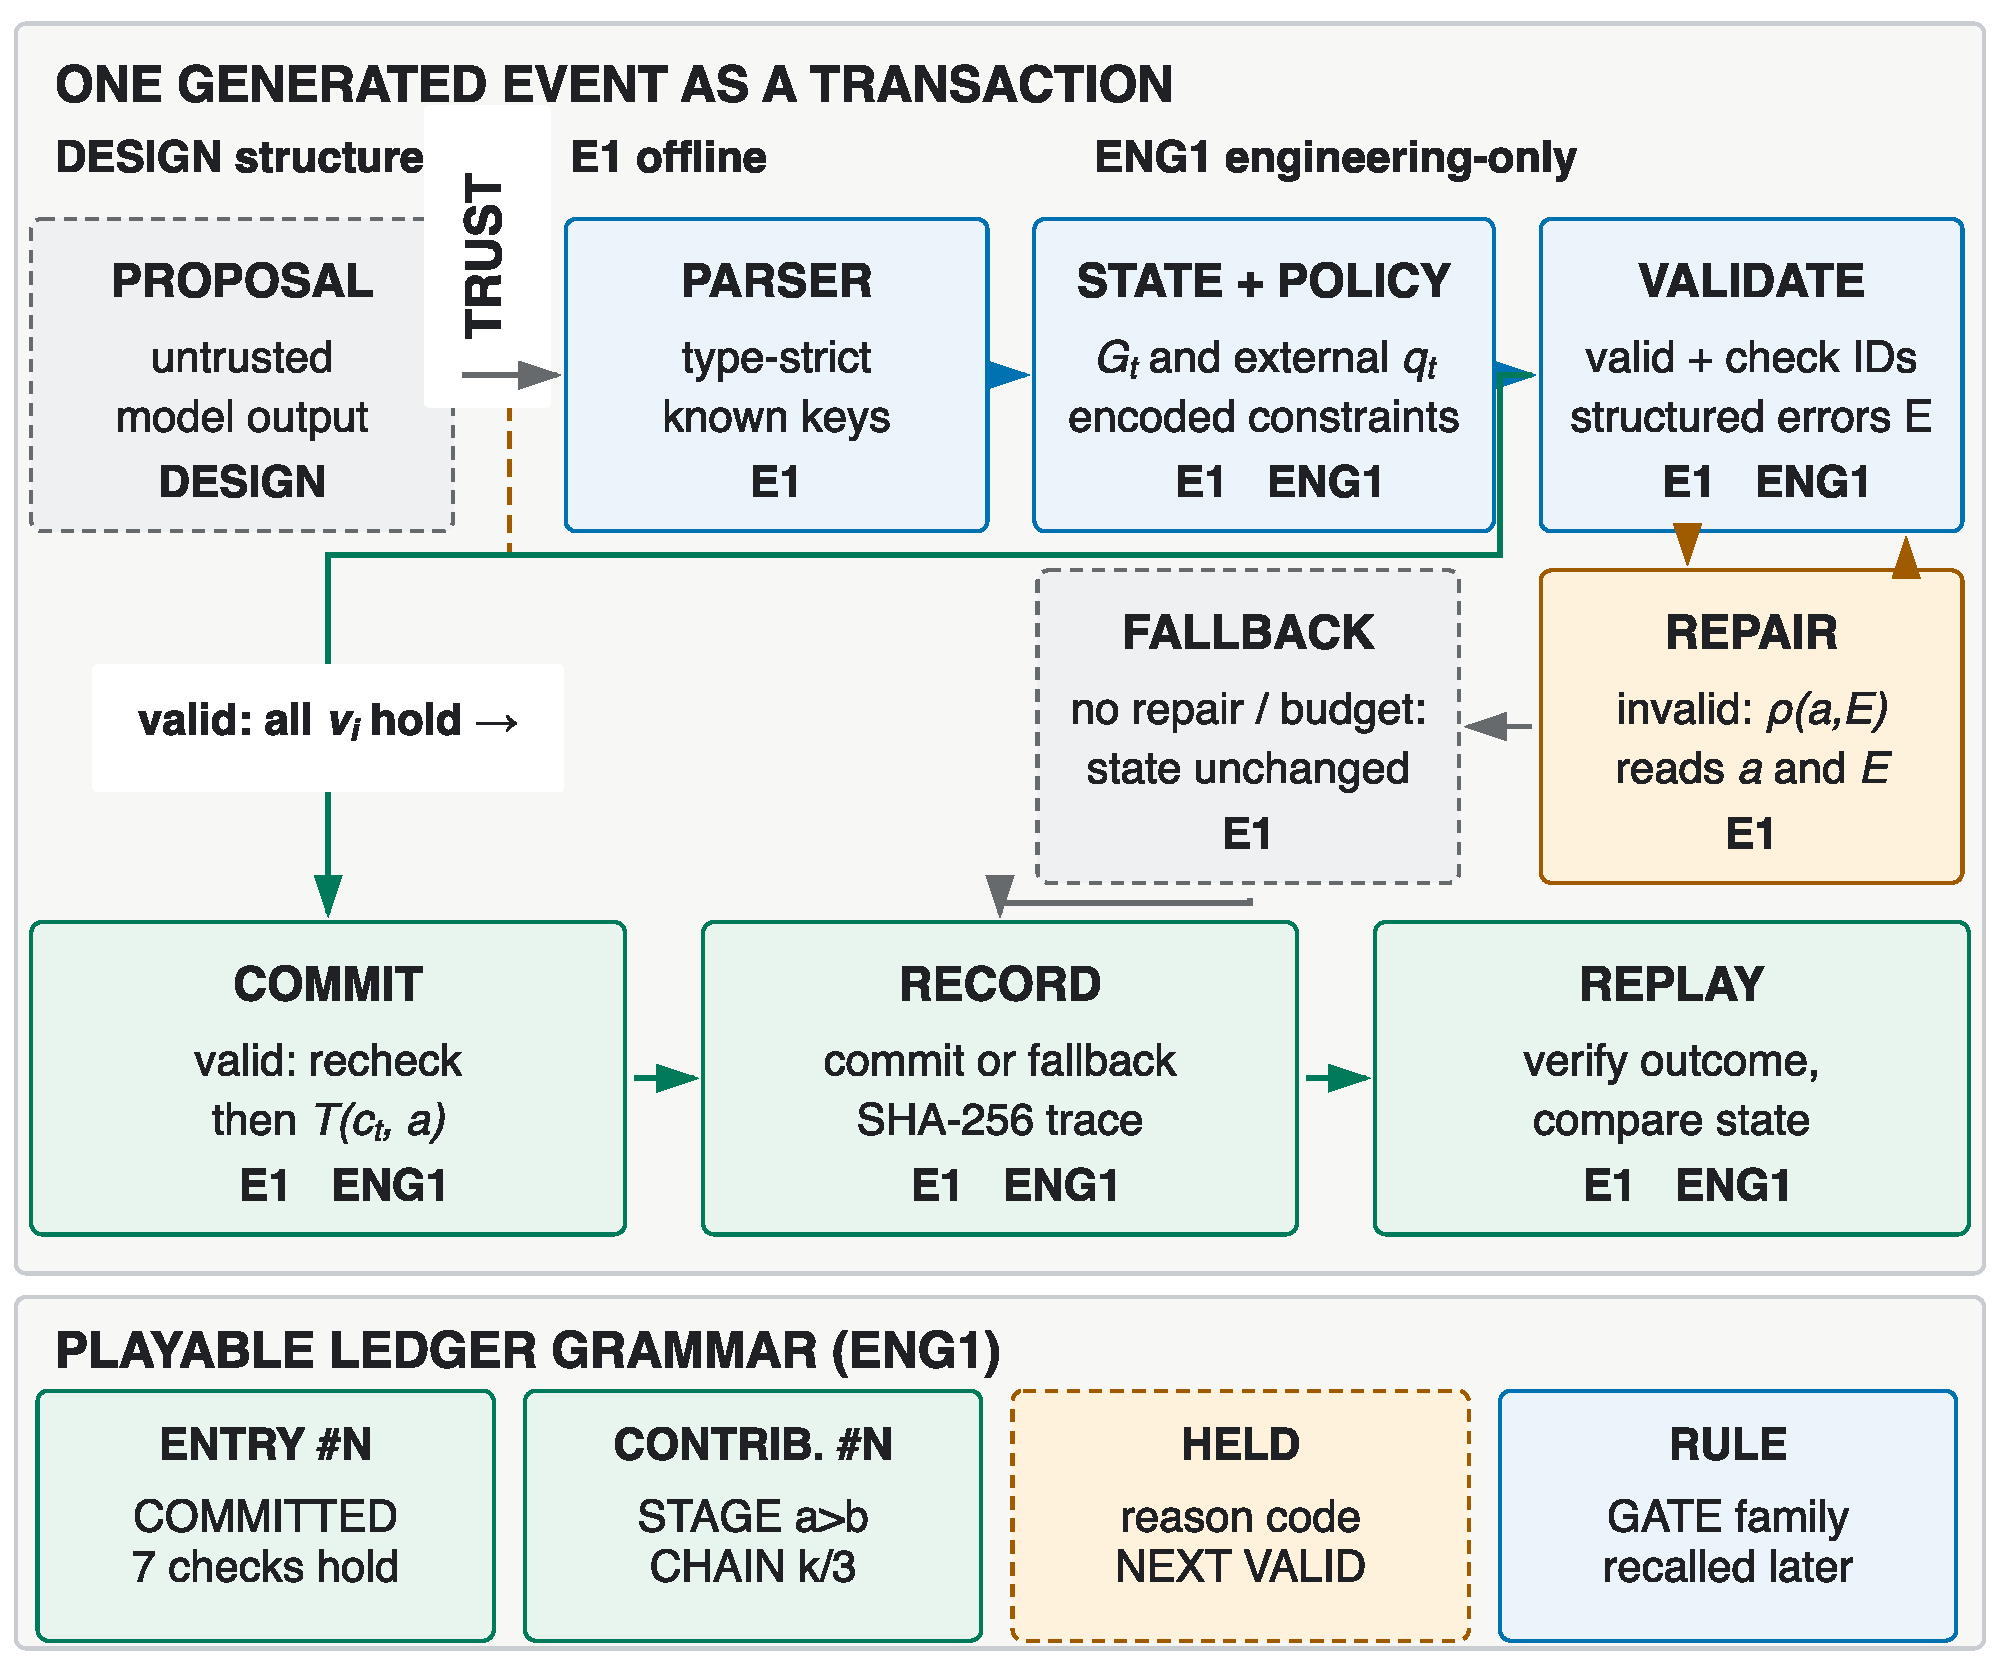
\includegraphics[width=0.72\textwidth]{../../figures/fig_architecture.pdf}
  \caption{정책과 상태 $c_t$가 제안을 게이팅하며, 오류는 $\rho$ 수리 또는 상태 불변 fallback으로 이어진 뒤 재검증을 거쳐 커밋된다.}
  \label{fig:architecture}
\end{figure*}

\section{문제 정의와 보장 경계}\label{sec:problem}
입력 $c_t=(G_t,q_t)$에서 $G_t$는 형식이 지정된 게임 스냅샷(장소, 도달 가능 위치, 물체 배치, 소지품, 사실, NPC 지식, 퀘스트 단계)을, $q_t$는 외부에서 저작된 행동 정책·정보 공개·퀘스트 단계 제약을 나타낸다. 검증 술어는 직전 이력 $h_{<t}$를 역산하거나 $q_t$를 변경하지 않으며, 검색 결과나 정서 점수는 쓰기 권한이 없다.

비신뢰 제안 $a_t$를 엄격히 파싱한 뒤, 검증기는 7개의 결정론적 술어를 실행하여 \texttt{ValidationResult}(\allowbreak$\mathrm{valid},E_t,C_{\mathrm{run}}$)를 반환한다:
\begin{equation}
\begin{aligned}
V(c_t,a_t)&=(\mathrm{valid},E_t,C_{\mathrm{run}}),\\
\boldsymbol{v}&=(v_{\mathrm{policy}},v_{\mathrm{pre}},v_{\mathrm{reach}},\\
&\qquad v_{\mathrm{know}},v_{\mathrm{disc}},v_{\mathrm{elig}},v_{\mathrm{stage}})\in\{0,1\}^{7},
\end{aligned}
\end{equation}
여기서 $\mathrm{valid}\equiv\bigwedge_{i=1}^{7}(v_i=1)$이며, $E_t$는 오류 코드·개체·원인·수리 힌트를 기록한다. 정본 상태는 7개 술어를 모두 통과한 경우에만 갱신된다:
\begin{equation}
c_{t+1}=\begin{cases}
T(c_t,a_t), & \bigwedge_{i=1}^{7}(v_i=1),\\
c_t, & \text{otherwise.}
\end{cases}
\label{eq:transition}
\end{equation}

\subsection{스키마 유효성, 권한, 목표 달성의 분리}\label{sec:authorization-sets}
행동 전 상태 $c_t$, 저작 정책, 엄격 스키마를 고정하고 스키마 유효 후보 집합을 $\SchemaSet$라 할 때, 권한과 목표 달성을 다음과 같이 분리한다:
\begin{equation}
\begin{aligned}
\AcceptSet(c_t)&=\{a\in\SchemaSet:V(c_t,a).\mathrm{valid}\},\\
\GoalSet(c_t)&=\{a\in\SchemaSet:\operatorname{Goal}(T(c_t,a))\},\\
\HitSet(c_t)&=\AcceptSet(c_t)\cap\GoalSet(c_t)\subseteq\AcceptSet(c_t)\subseteq\SchemaSet.
\end{aligned}
\end{equation}
금지 사실을 선언한 스키마 유효 후보는 $\AcceptSet$ 밖에 놓이며, 허용된 관찰 행동은 $\AcceptSet$에 속하지만 $\GoalSet$ 밖에 놓일 수 있다. 지식과 공개 권한은 독립 입력이다. 예컨대 NPC는 0단계와 1단계 모두에서 \texttt{keeper\_\allowbreak secret}을 알고 있으나, 공개는 0단계에서 금지되고 1단계에서 허용된다.

\subsection{불변식 I1--I4에 대한 형식 안전성 정리}\label{sec:formal-proofs}
결정론적 전이 규칙(식~\eqref{eq:transition})과 엄격 파서 \texttt{parse\_}\allowbreak\texttt{candidate\_}\allowbreak\texttt{mapping} 아래에서 불변식 \textbf{I1--I4}는 임의의 유한 인코딩 상태 $c_t=(G_t,q_t)$, 수리 예산 $K\in\mathbb{Z}_{\geq 0}$ 및 정상 반환 콜백에 대한 조건부 구조 정리로 성립한다.

\noindent\textbf{정리 1 (I1: 상태 보존 안전성).} \emph{초기 후보가 엄격 파싱을 통과하지 못하거나 $K{+}1$회 모든 시도에서 $V(c_t,a^{(j)}).\mathrm{valid}=\mathrm{false}$이면 $c_{t+1}=c_t$이며 커밋된 효과는 비어 있다.}
\par\noindent\textit{증명.} \texttt{parse\_}\allowbreak\texttt{candidate\_}\allowbreak\texttt{mapping}은 커밋 전에 비정형 제안을 거부하며, 그림~\ref{alg:commit}에서 $\operatorname{Commit}$은 $\mathrm{ok}=\mathrm{true}$일 때만 도달 가능하고 $j=K$에서는 $\operatorname{Fallback}(c_t)$이 식~\eqref{eq:transition}에 의해 $c_t$를 그대로 반환한다. \hfill$\square$

\noindent\textbf{정리 2 (I2: 유한 종료와 상태 비참조 세탁 방지 수리).} \emph{유한 $K{\geq}0$과 정상 반환 콜백 하에서 루프는 $V$를 최대 $K{+}1$회 호출하며, 상태 변경 직전 $V(c_t,a^{(j)})$를 재검증하고, $\rho$는 \texttt{WorldState} 의존 권한 오류 클래스를 변경하지 않는다.}
{\sloppy\par\noindent\textit{증명.} 계수기 $j$는 $0$에서 시작하여 증가 전 $j=K$를 검사하므로 $V$ 호출은 최대 $K{+}1$회로 유계다. 표~\ref{tab:rho-rules}에 따라 $\rho(a,E)$는 \texttt{WorldState}를 읽지 않고 $(a,E)$만 입력받아 \texttt{UNKNOWN\_}\allowbreak\texttt{ACTION\_}\allowbreak\texttt{TYPE}, \texttt{UNREACHABLE\_}\allowbreak\texttt{REQUIRED\_}\allowbreak\texttt{OBJECT}, \texttt{NPC\_}\allowbreak\texttt{KNOWLEDGE\_}\allowbreak\texttt{VIOLATION}, \texttt{NPC\_}\allowbreak\texttt{DIS\-CLOSURE\_}\allowbreak\texttt{KNOW\-LEDGE\_}\allowbreak\texttt{VIO\-LATION}, \texttt{FORBIDDEN\_}\allowbreak\texttt{DISCLOSURE}, \texttt{QUEST\_}\allowbreak\texttt{STAGE\_}\allowbreak\texttt{VIOLATION}, \texttt{QUEST\_}\allowbreak\texttt{STAGE\_}\allowbreak\texttt{REGRESSION}을 항등 사상으로 두고 동일 필드 상충 편집을 제거한다. \hfill$\square$\par}

\noindent\textbf{정리 3 (I3: 정책 유계 상태 변이).} \emph{커밋된 모든 전이는 7개 술어 $v_1\dots v_7$을 만족하며 \texttt{ActionPolicy.}\allowbreak\texttt{allowed\_}\allowbreak\texttt{effects}에 허용된 효과만 반영한다.}
\par\noindent\textit{증명.} 엄격 파서가 12개 \texttt{CANDIDATE\_}\allowbreak\texttt{FIELDS}를 동결하고, $v_{\mathrm{policy}}{=}1$이 허용 집합 포함 여부를 검증하며, $T$는 선언 외 키를 기록하지 않는다. \hfill$\square$

\noindent\textbf{정리 4 (I4: 결정론적 의미 리플레이 및 변조 탐지).} \emph{\texttt{allow\_}\allowbreak\texttt{defaults=}\allowbreak\texttt{false} 파싱과 동결 $(V,T)$ 하에서 정렬된 해시 연쇄 전이 기록을 $c_0$부터 재실행하면 $c_T$가 유일하게 복원되며 단일 단계 변조도 SHA-256 연쇄 불일치로 탐지된다.}
\par\noindent\textit{증명.} $V,T$는 $(c_t,a_t)$의 순수 결정론적 함수이고 각 기록은 $(\mathrm{hash}(c_t),\allowbreak a_t,\allowbreak V(c_t,a_t),\allowbreak\mathrm{hash}(c_{t+1}))$을 해싱하므로 귀납적으로 $\mathrm{hash}(c'_T)=\mathrm{hash}(c_T)$가 일치한다. \hfill$\square$

\section{TRACE-RPG 아키텍처와 알고리즘}\label{sec:arch}
모델과 어댑터가 후보 행동을 제안하면 엄격 파서가 미등록 키와 모호한 타입을 거부하고, 버전 관리 브리지가 관측·제안·검증·거부·대체(fallback)·커밋을 전달한다(그림~\ref{fig:architecture}, 표~\ref{tab:validators}). 여덟 역할 읽기 전용 온톨로지 뷰(\texttt{World}, \texttt{Actor}, \texttt{Knowledge}, \texttt{Fact}, \texttt{Policy}, \texttt{Quest}, \texttt{Action}, \texttt{Trace})는 쓰기 권한 없이 출처 선언을 실행 검사 및 리플레이 영수증에 연결한다.

\begin{table}[!tbp]
\caption{인코딩된 7술어 검증기 경계}
\label{tab:validators}
\centering
\footnotesize
\begin{tabularx}{\columnwidth}{@{}>{\raggedright\arraybackslash}p{0.25\columnwidth}>{\raggedright\arraybackslash}X>{\raggedright\arraybackslash}p{0.16\columnwidth}@{}}
\toprule
\textbf{술어} & \textbf{거부 조건} & \textbf{실패 시} \\
\midrule
행동 정책 & 미등록 행동/유형, 필수 조건·효과 누락, 비허용 효과 & 상태 불변 \\
선행조건 & 부재 또는 거짓인 필수 조건 & 상태 불변 \\
도달 가능성 & 접근 불가능한 대상 물체 & 상태 불변 \\
NPC 지식 & 행위자 지식에 없는 사실 사용·공개 & 상태 불변 \\
정보 공개 & 선언된 금지 사실 포함 & 상태 불변 \\
퀘스트 단계 & 현재 단계보다 높은 요구 단계 & 상태 불변 \\
단계 단조성 & 역행하는 퀘스트 단계 전이 & 상태 불변 \\
\bottomrule
\end{tabularx}
\end{table}

\begin{figure}[!tbp]
\centering
\footnotesize
\begin{tabular}{@{}rl@{}}
1: & $a\leftarrow\operatorname{Propose}(c)$; $j\leftarrow0$ \\
2: & \textbf{repeat} \\
3: & \quad $(\mathrm{ok},E)\leftarrow V(c,a)$; $\operatorname{Record}(a,E)$ \\
4: & \quad \textbf{if} $\mathrm{ok}$ \textbf{then assert} $V(c,a).\mathrm{ok}$; \textbf{return} $\operatorname{Commit}(c,a)$ \\
5: & \quad \textbf{if} $j=K$ \textbf{then return} $\operatorname{Fallback}(c)$ \\
6: & \quad $a\leftarrow\operatorname{Repair}(c,a,E)$; $j\leftarrow j+1$ \\
7: & \textbf{until terminal}
\end{tabular}
\caption{검증--수리--커밋 루프는 최대 $K+1$회 시도를 기록하고 커밋 직전에 재검증한다.}
\Description{최대 K+1회 시도를 기록하고 커밋 직전 재검증하는 검증-수리-커밋 루프 의사코드.}
\label{alg:commit}
\end{figure}

유도 수리 연산자 $\rho(a,E)=a\oplus\bigcup_{e\in E}\delta(e)$(그림~\ref{alg:commit}, 표~\ref{tab:rho-rules})는 \texttt{WorldState}를 전혀 읽지 않고 후보 $a$와 구조 오류 $E$만 입력받아 도달 가능성·지식·공개 위반의 우회 세탁(state laundering)을 차단한다. 전이 기록은 이전 상태, 후보, 검증 결과, 재계산된 최종 상태에 대해 비키(unkeyed) SHA-256 해시를 연쇄 기록하여 결정론적 의미 리플레이와 배정 전수 분모 계수를 지원한다.

\begin{table}[!tbp]
\caption{유도 수리 연산자 $\rho(a,E)$의 오류 유형별 편집 규칙}
\label{tab:rho-rules}
\centering
\footnotesize
\begin{tabularx}{\columnwidth}{@{}>{\raggedright\arraybackslash}X>{\raggedright\arraybackslash}X@{}}
\toprule
\textbf{검증기 오류 유형} & \textbf{후보 $a$에 대한 편집 $\delta(e)$} \\
\midrule
정책 선행조건 / 효과 누락 & 명시된 술어 또는 효과 삽입 \\
정책 효과 위반 & 비허용 효과 제거 \\
불만족 선행조건 & 명시된 술어 제거 \\
비인가 단계 변경 & \texttt{quest\_stage\_effect} 초기화 \\
미등록 행동; 도달·지식·공개·단계 오류 & 무연산(no-op, 상태 세탁 방지) \\
\bottomrule
\end{tabularx}
\end{table}

\section{평가}\label{sec:eval}
평가는 서로 통합(pooling)하지 않는 두 계층으로 구성된다: (i) 유한 그래프, 공개 행렬, 링크 예측 시뮬레이션, Godot~4.7.1 엔진 실행에 대한 0-LLM 결정론적 감사 계층, (ii) 배정 전수 분모를 유지하는 제한된 확률적 제안기 파일럿 계층.

\subsection{결정론적 권한 경계 감사}
단일 월드 단위 픽스처를 넘어 권한 경계를 검증하기 위해, 방 개수 2종(4, 8), 위상 2종(잠긴 연쇄, 비잠금 우회 분기), 재사용 열쇠 2개의 시작/목표 배치 4종, 퀘스트 단계 2종을 교차한 $2{\times}2{\times}4{\times}2=32$개 그래프-상태 조합에 후보 변형 13종을 적용해 조건당 416건(총 1,664건)을 배정하고, 별도로 표면 센티넬 48건(조건당 12건)을 구성했다. 구현이 분리된 기준 검증기가 표준 라이브러리 BFS 도달 가능성을 사용해 불변의 행동 전 상태에 대해 초기 및 수리 후보를 판정했다.

\begin{table}[!tbp]
\caption{결정론적 권한 경계 감사 (조건당 416건 + 표면 센티넬 48건; 0 LLM 호출)}
\label{tab:boundary-compact}
\centering
\footnotesize
\begin{tabularx}{\columnwidth}{@{}>{\raggedright\arraybackslash}X*{4}{>{\centering\arraybackslash}p{0.11\columnwidth}}@{}}
\toprule
\textbf{결과 (416/조건)} & \textbf{스키마} & \textbf{거부} & \textbf{재시도} & \textbf{유도 $\rho$} \\
\midrule
최초 무효 제안 & 260 & 260 & 260 & 260 \\
위험 최종 커밋 & 260 & \textbf{0} & \textbf{0} & \textbf{0} \\
수리 복구 (무효$\rightarrow$유효) & 0 & 0 & 0 & \textbf{128} \\
보류 (상태 불변) & 0 & 260 & 260 & 132 \\
목표 달성 & 124 & 124 & 124 & \textbf{252} \\
최초 유효 보존 (156건) & 156 & 156 & 156 & 156 \\
구조 서명 보존 (11종) & 11/11 & 11/11 & 11/11 & 11/11 \\
\bottomrule
\end{tabularx}
\end{table}

표~\ref{tab:boundary-compact}에서 \texttt{schema\_only}는 기준상 무효인 제안 260/416건을 모두 커밋한 반면, 모든 의미 게이트 조건은 오탐 0/156건과 폐쇄--BFS 32/32 일치 속에 0/416건만 커밋했다. 유도 수리 $\rho$는 무효 제안 128/260건을 복구해 목표 달성을 124/416건에서 252/416건으로 거의 두 배 높였다. 표면 센티넬 12건/조건에서는 명시적 금지 사실 6/6건을 모두 차단했으나 미선언 우회 표현 6/6건을 통과시켜 선언 필드 기반 게이트의 정확한 한계를 정량화했다.

\subsection{정보 공개 동등성과 온톨로지 링크 시뮬레이션}
저작된 \texttt{reveal\_hint} 60건(정상 48, 경계 4, 비정상 8)에서 비검증 대조군은 51건의 고유 위험 공개(60/60 허용)를 발생시켰으나, \texttt{general\_rule}과 \texttt{ontology\_gate}는 60/60건에서 완전히 일치(허용 16, 거부 44, 위험 0, 리플레이 불일치 0)했다. 이는 온톨로지의 우위가 아니라 무회귀 감사 바인딩을 입증한다. 별도로 닫힌 세계 KG 링크 제안 시뮬레이션(43 OKF 노드, 106 참조 에지, 24 큐레이션 타입 에지, 6 보류 에지 질의)에서 타입-어휘 검색(\texttt{S2})은 $P{=}R{=}1.000$, $\mathrm{MRR}{=}0.944$, $\mathrm{Sem@3}{=}1.000$을 기록했다(차수 기준선 $P{=}R{=}0.000$, $\mathrm{MRR}{=}0.282$).

\subsection{확장 0-LLM 공학 감사 (A1--A4, B)}
표~\ref{tab:extended-compact}은 다중 오류 수렴, 스케일링, 추적성, Godot~4.7.1 장기 안정성, 2차 우회 필터를 다루는 독립 분모 결정론적 감사 5종을 요약한다.

\begin{table*}[!tbp]
\caption{독립 분모 0-LLM 공학 감사 요약 (A1--A4, B)}
\label{tab:extended-compact}
\centering
\footnotesize
\begin{tabularx}{\textwidth}{@{}>{\raggedright\arraybackslash}p{0.20\textwidth}>{\raggedright\arraybackslash}p{0.21\textwidth}>{\raggedright\arraybackslash}X@{}}
\toprule
\textbf{감사 항목} & \textbf{독립 분모 / 범위} & \textbf{검증된 결정론적 결과 (0 LLM 호출)} \\
\midrule
\textbf{A1} 다중 오류 수렴 & 예산당 352건 ($K{\in}\{0..3\}$, 1,408실행) + 128가드 & 안전 커밋: $K{=}0$ 0/352, $K{\ge}1$ 124/352 (35.23\%, 위험 0/1,408); \texttt{repairable\_multi} 96/96 ($K{=}1$); \texttt{conflict\_pair} 교차 시도 0/96 (주기-2 진동 96/96) vs.\ 동일 패스 가드 128/128 동결. \\
\textbf{A2} 지연 스케일링 & $N{\in}[10,2000]$ 사실 ($N{>}500$서 차수$\le$100), $R{\in}[4,256]$ 방 & $N{=}2000$ 기준 검증기 p95 0.0042\,ms (유효) / 0.0751\,ms (다중오류); $\rho$ p95 0.0317--0.0389\,ms; $R{=}256$ 폐쇄/BFS p95 0.312--0.478\,ms; SHA-256 검증 7.01\,ms; JSONL 리플레이 881.0\,ms. \\
\textbf{A3} 추적성 결함 & 시드 결함 4,656건(+N/A 1,584), 불변 3,744, \texttt{TR05} & 시드 결함 민감도 4,656/4,656 (100.00\%); 불변 오경보 0/3,744 (0.00\%); \texttt{TR05} 정방향 12/12, 역방향 10/10 직접 파일; 인간 Krippendorff $\alpha$ 미측정 (평가자 0명). \\
\textbf{A4} Godot~4.7.1 장기 실행 & 거부 코드 11건 + 1,600틱 (200에피소드) & 거부 코드 9/9 (100\%) 실행; 상태 격리 11/11; 트레이스 일관성 1,600/1,600; \texttt{step\_commit} p95 0.708\,ms; 정적 메모리 증감 $-268$\,B; 누수 0건. \\
\textbf{B} 우회 필터 (영/한) & 88건 (영 44, 한 44; \texttt{keeper\_secret}) & 재현율 / 양성 오거부율(FRR) / p95: ID전용 0.0\% / 0.0\% / 0.032\,ms; 별칭 61.1\% (22/36) / 11.1\% (4/36) / 0.041\,ms; LOO TF-IDF 97.2\% (35/36) / \textbf{58.3\% (21/36)} / 0.705\,ms. \\
\bottomrule
\end{tabularx}
\end{table*}

\subsection{제한된 확률적 제안기 파일럿}
두 소규모 비확증적 파일럿에서는 모든 파서 및 하네스 실패를 분모에 그대로 보존한다:
\begin{itemize}
\item \textbf{v5 2단계 수집 (배정 20건):} 합성 픽스처 5종 $\times$ 셀렉터 2종 $\times$ Detailed/Generic 피드백($K{=}0$)에서 20/20건 수신, 10/20건 엄격 파싱 통과(Luna 9/10, Terra 1/10), 8/20건 의미 게이트 통과(거부된 2건 상태 불변), 7/20건이 \texttt{signal\_restored}에 도달했다(그림~\ref{fig:paired-feedback-flow}).
\item \textbf{네이티브 단일 퀘스트 파일럿 (배정 8건):} \texttt{sealed-}\allowbreak\texttt{lighthouse-}\allowbreak\texttt{v1}($2{\times}2{\times}2$)에서 5/8건 목표 달성, 위험 커밋 0/16, 의미 리플레이 7/7 유효, 신규 Godot 재실행 6/6 유효를 기록했다(행 1의 controller-v3 직렬화 오류 1건은 행 2--8에서 v4로 수정, 온톨로지 행 2건은 60초 타임아웃).
\end{itemize}

\begin{figure}[!tbp]
\centering
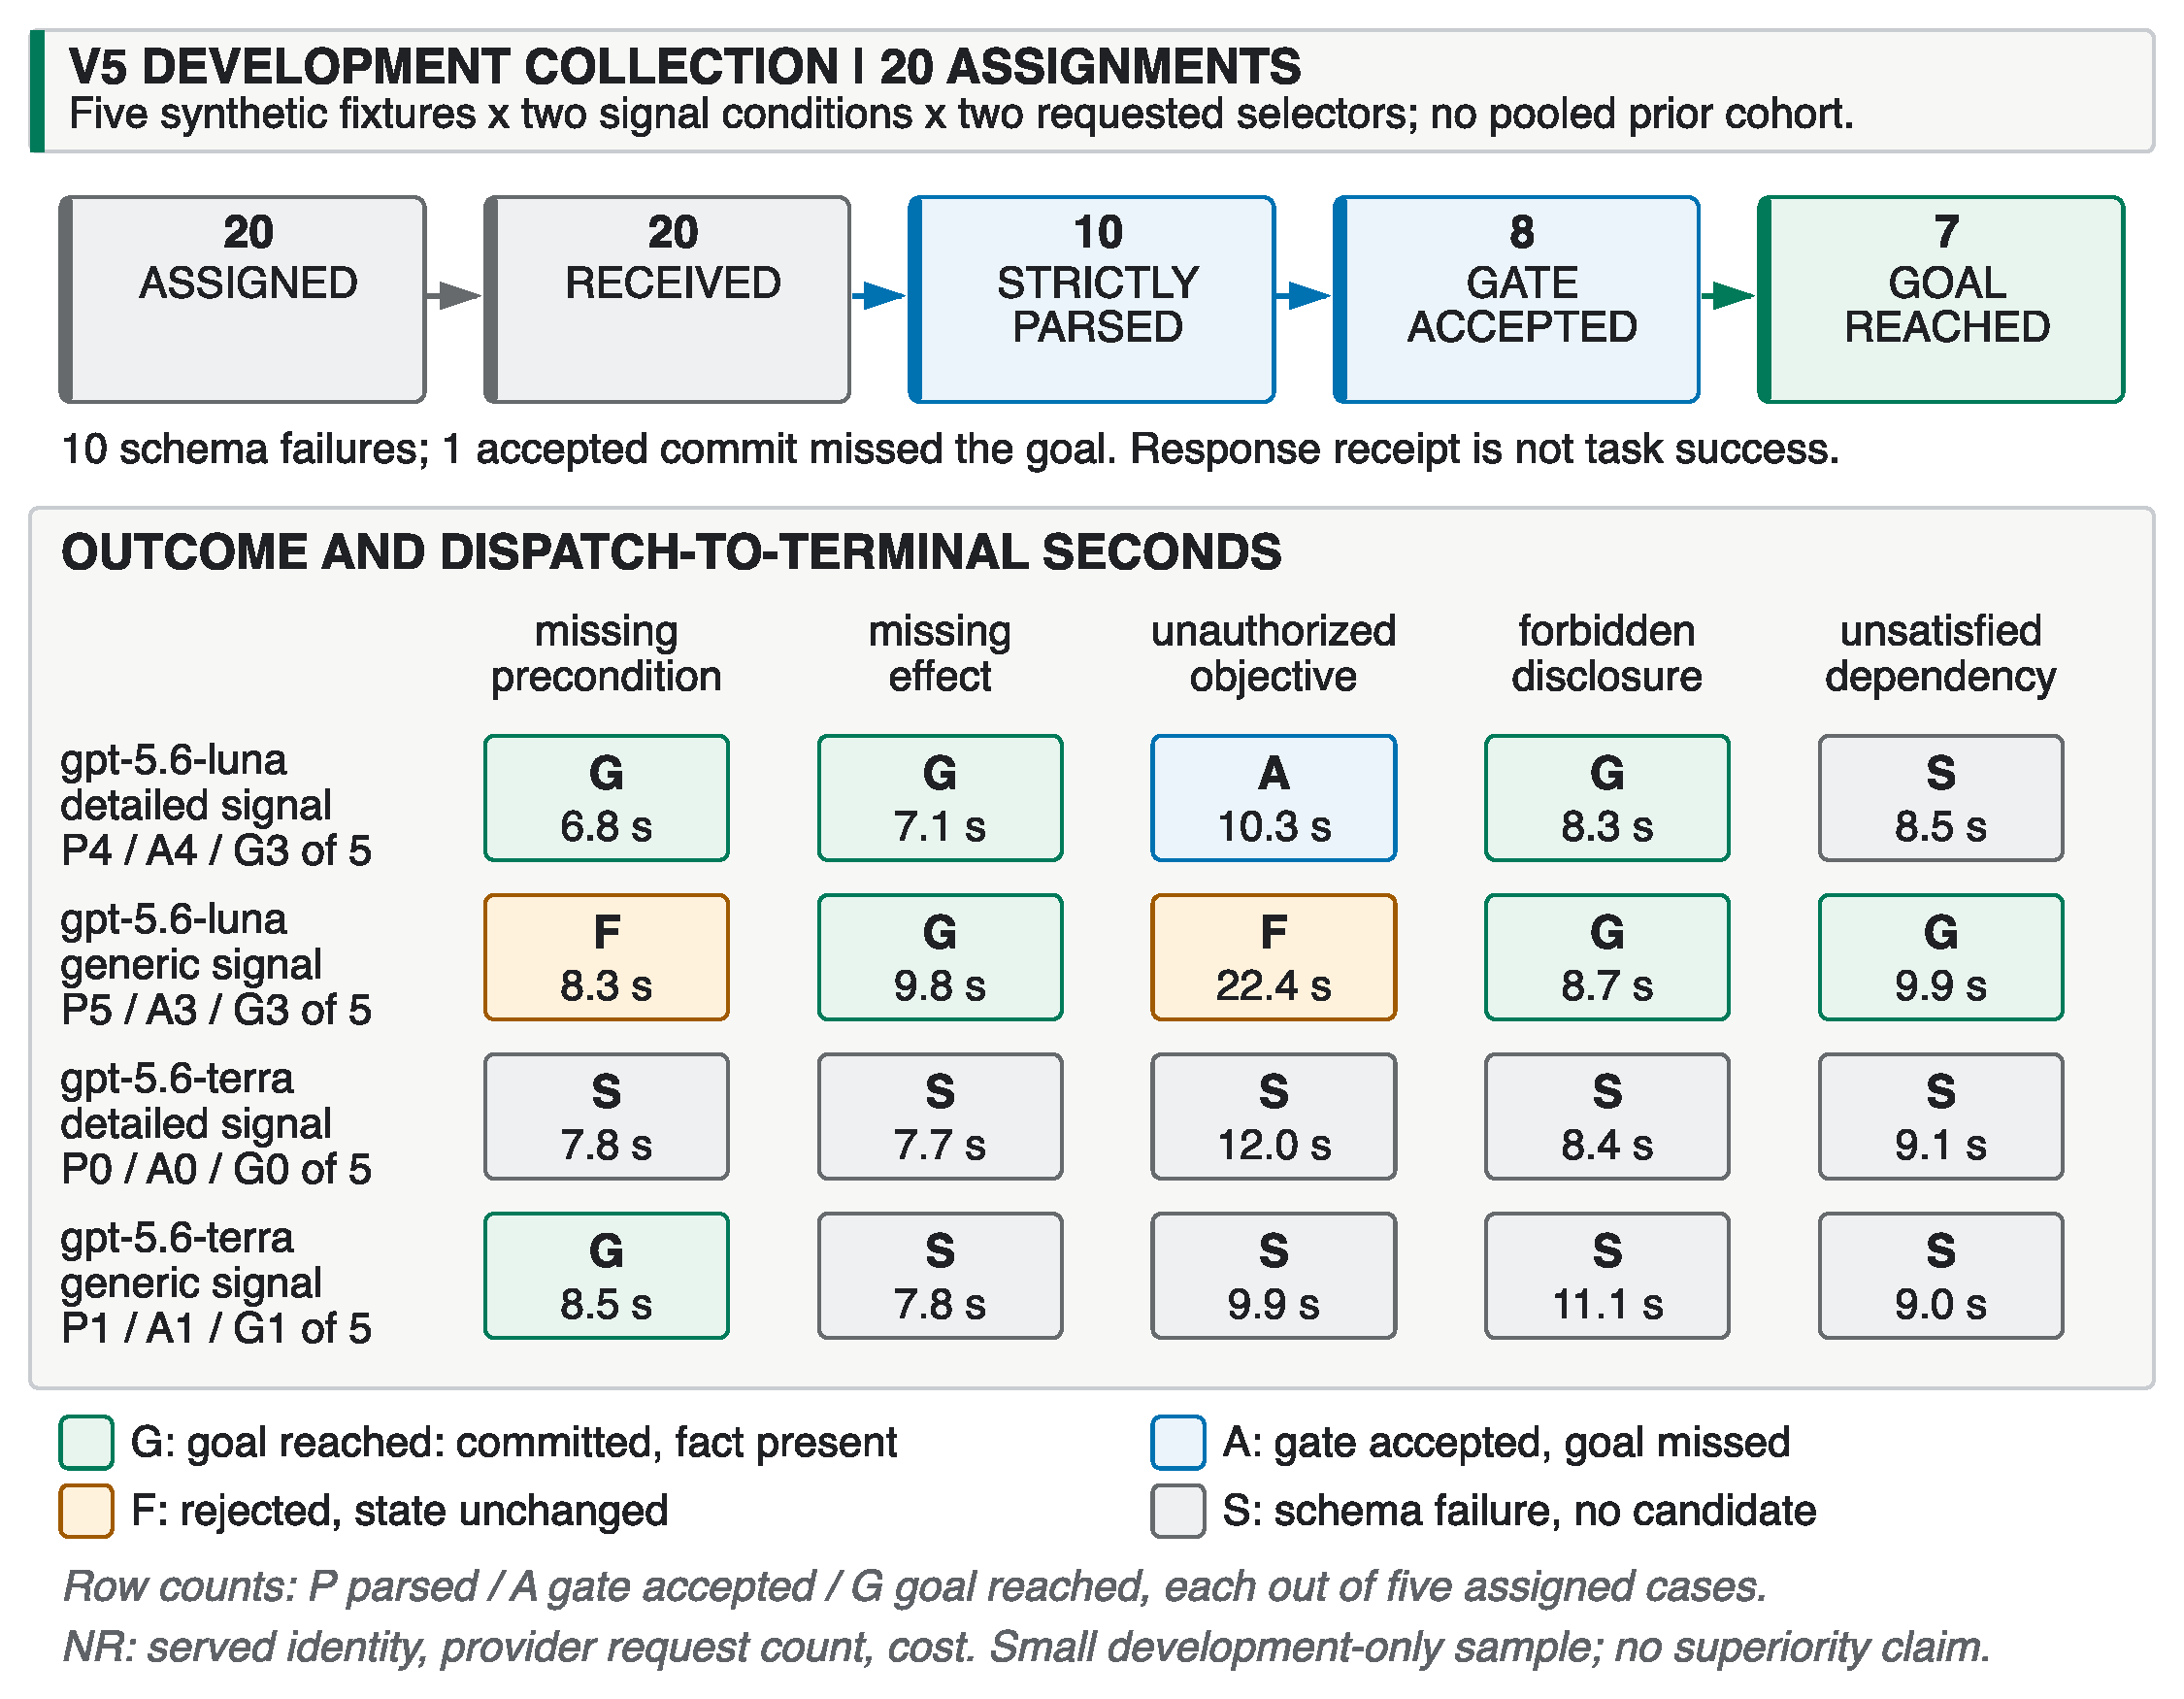
\includegraphics[width=\columnwidth]{../../figures/fig_paired_feedback_flow.pdf}
\caption{v5 배정 20건 전체 결과 흐름: 스키마 실패 10건을 분모에 보존하며, 게이트 통과 8건 중 7건이 목표에 도달했다.}
\Description{v5 배정 20건 결과 흐름도: 스키마 실패 10건, 게이트 통과 8건, 목표 달성 7건.}
\label{fig:paired-feedback-flow}
\end{figure}

\subsection{다중 홉 폐쇄, 라이브 다중 퀘스트, 2차 우회 검증기}\label{sec:green-supplements}
표~\ref{tab:green-venue-compact}은 네 가지 추가 보강 검증을 요약한다. 첫째, 3개 퀘스트 그래프의 48건 다중 홉 폐쇄 벤치마크(1홉 16, 파생 16, 역할 상속 16)에서 \texttt{flat\_}\allowbreak\texttt{1hop\_}\allowbreak\texttt{rule}은 위험 전이 28건을 누출(정확도 41.7\%, 20/48)했으나 \texttt{ontology\_}\allowbreak\texttt{multihop\_}\allowbreak\texttt{gate}는 100.0\%(48/48, 누출 0건)를 달성하고 \textbf{I1--I4}를 통과해 60/60 단일 홉 동률을 넘어섰다. 둘째, 격리 샌드박스 Antigravity CLI 라이브 평가(\texttt{cli\_version~1.5.11}, 엄격 \texttt{--json-schema}, $K{\in}\{0..2\}$, 제공자 리비전·시드 미인증) 24에피소드에서 두 Gemini 모델 모두 위험 커밋 0/129건과 엄격 리플레이 24/24건을 기록했으며, 스키마 통과 후 위험 턴 70건을 차단했다(실패 71건 중 69건이 수리 불가 \texttt{NPC\_}\allowbreak\texttt{KNOWLEDGE\_}\allowbreak\texttt{VIOLATION}으로 정리~2에 따라 수리 0회). 셋째, 한·영 Audit~B 88건 전체에서 \texttt{rule\_hybrid}는 FRR을 58.3\%에서 2.8\%로 낮췄고($F_1{=}0.809$), 라이브 2차 \texttt{gemini-3.8-}\allowbreak\texttt{flash-}\allowbreak\texttt{medium}은 우회 재현율 97.2\%(35/36)와 0.0\% FRR($F_1{=}0.990$, 파싱 오류 0건)을 달성했다(탐색적 로컬 0.8B 자문 기준선 0/36 대비). 넷째, 트레이스 결속 36항목 \texttt{TR01--TR06} 패킷(\texttt{AWAITING\_}\allowbreak\texttt{HUMAN\_}\allowbreak\texttt{RATERS}, $N{=}0$, 합성 라벨 0건)과 Croissant~1.0 메타데이터(6/6 SHA-256 일치)를 구축했다.

\begin{table}[!tbp]
\caption{다중 홉 폐쇄, 라이브 다중 퀘스트 Gemini 및 2차 Audit~B 보강 요약}
\label{tab:green-venue-compact}
\centering
\scriptsize
\begin{tabularx}{\columnwidth}{@{}>{\raggedright\arraybackslash}p{0.27\columnwidth}>{\raggedright\arraybackslash}X@{}}
\toprule
\textbf{보강 축} & \textbf{검증 결과 (전체 분모 보존)} \\
\midrule
다중 홉 폐쇄 (48건, 3월드) & \texttt{flat\_}\allowbreak\texttt{1hop\_}\allowbreak\texttt{rule}: 41.7\% (9 TP, 11 TN, 누출 28); \texttt{ontology\_}\allowbreak\texttt{multihop\_}\allowbreak\texttt{gate}: \textbf{100.0\%} (37 TP, 11 TN, 누출 0); I1--I4 통과. \\
라이브 \texttt{gemini-3.8-}\allowbreak\texttt{flash-}\allowbreak\texttt{medium} (12 ep) & 목표 7/12 (일반 4/6, 온톨로지 3/6); 커밋 36/57; 차단 21; \textbf{위험 0}; 리플레이 12/12; 파싱오류 0; 1.99M tok. \\
라이브 \texttt{gemini-4-}\allowbreak\texttt{hydrogen-}\allowbreak\texttt{medium} (12 ep) & 목표 0/12; 커밋 21/72; 차단 49; \textbf{위험 0}; 리플레이 12/12; 타임아웃 2건 보존; 2.62M tok. \\
2차 우회 한·영 (88건) & \texttt{rule\_hybrid}: 우회 55.6\% / FRR 2.8\% / $F_1{=}0.809$; 라이브 Flash: \textbf{97.2\% (35/36) / FRR 0.0\%} / $F_1{=}0.990$; Hydrogen: 80.6\% / FRR 0.0\% / $F_1{=}0.928$ (오류 9). \\
인간·데이터 준비 & \texttt{TR01--TR06} 36항목 실제 트레이스 결속 (\texttt{AWAITING\_}\allowbreak\texttt{HUMAN\_}\allowbreak\texttt{RATERS}, 0 합성); Croissant~1.0 (6/6 SHA-256). \\
\bottomrule
\end{tabularx}
\end{table}

\FloatBarrier
\section{타당성 위협, 한계 및 결론}\label{sec:conclusion}
\textbf{한계와 타당성 위협.} 다중 홉 보강으로 평가 세계를 1개에서 3개 퀘스트로 확장하고 60/60 평면 규칙 동률을 돌파했으며(\texttt{ontology\_}\allowbreak\texttt{multihop\_}\allowbreak\texttt{gate} 100.0\% 대 \texttt{flat\_}\allowbreak\texttt{1hop\_}\allowbreak\texttt{rule} 41.7\%, 48건), 2차 Gemini 검증기가 Audit~\textbf{B} 오거부율(FRR)을 58.3\%에서 0.0\%로 낮췄음에도 네 가지 경계가 남는다. 첫째, 라이브 Antigravity CLI Gemini 실험($n{=}24$ 다중 퀘스트, $n{=}88{\times}2$ Audit~B)은 제공자 리비전·시드 미인증과 타임아웃 11건(에피소드 2, Audit~B Hydrogen 9)을 분모에 그대로 유지하며, 비공개 모델 성능 우위가 아닌 래퍼 안전성을 입증한다. 둘째, 사전 등록 180단위 다중 모델 프로토콜은 인증된 API 키 부재로 \texttt{0/180}(\texttt{NOT\_RUN/BLOCKED}) 상태다. 셋째, 3개 퀘스트 월드(\texttt{sealed-}\allowbreak\texttt{lighthouse-}\allowbreak\texttt{v1}, \texttt{sunken-}\allowbreak\texttt{archive-}\allowbreak\texttt{v1}, \texttt{clockwork-}\allowbreak\texttt{observatory-}\allowbreak\texttt{v1})는 대규모 상용 엔진이 아닌 소형 상태 기계다. 넷째, 인간 평가($N{=}0$)는 미실행 상태다: \texttt{TR01--TR06} 36항목 블라인드 패킷은 해시 검증 상태로 구축되었으나 \texttt{AWAITING\_}\allowbreak\texttt{HUMAN\_}\allowbreak\texttt{RATERS}(합성 라벨 0건)이므로 사용성·몰입감·Krippendorff~$\alpha$는 후속 인간 평가가 필요하다.

\textbf{결론.} \system{}는 7술어 검증기, 반례 유도 수리 $\rho(a,E)$, 해시 연결 의미 리플레이, 읽기 전용 8역할 온톨로지 관측을 통해 제안 권한과 커밋 권한을 분리한다. 조건부 정리 1--4가 불변식 \textbf{I1--I4}를 증명하고, 다중 홉 폐쇄가 평면 규칙 누출 28/48건을 제거하며, 24개 라이브 Gemini 에피소드 및 2차 우회 검증이 위험 커밋 0/129건, 위험 턴 70건 차단, 엄격 리플레이 24/24건, FRR 0.0\%(우회 재현율 97.2\%)을 입증해 향후 인증된 180단위·인간 평가의 토대를 완성한다.

\section*{윤리 및 아티팩트 공개}
초고·코드·테스트 작성에 대규모 언어 모델의 보조를 받았으며 모든 주장, 인용, 정리 1--4 및 결정론적·라이브 산출물(Croissant~1.0 메타데이터 포함)은 저자가 검증하였고 인간 라벨은 일절 합성하지 않았다. 저장소 주소: \RepoURL.


\FloatBarrier
\bibliography{../../references}

\end{document}
